\documentclass{article}
\usepackage{amsmath}
\usepackage{graphicx}
\usepackage{float}
\usepackage{subcaption}

\begin{document}
\title{Camera calibration}
\author{Haochen Feng \\uid: u6927368} 
\date{\today}
\maketitle

\section*{Introduction}
\noindent
For the camera calibration process, 
we describe the calibration process of the 
camera and the Inertial Measurement Unit (IMU) 
using both the data obtained from driving 
the car and the OpenCV Python library. 
The calibration process involves determining the IMU frame, 
camera frame, IMU rotation, and IMU translation. 
The goal of the calibration is to accurately 
estimate the transformation between the camera and 
IMU coordinate frames (extrinsic matrix) and the 
camera's intrinsic matrix. The intrinsic matrix 
contains information about the camera's internal 
characteristics, such as focal length ($f_x, f_y$) and principal point($c_x, c_y$). 
The quality of the calibration will 
be assessed by calculating the reprojection error, 
which is a measure of how well the estimated parameters 
map 3D world points to their corresponding 2D image points. 
A low reprojection error indicates 
a successful calibration, 
enabling accurate data fusion between the camera 
and IMU for applications such as visual-inertial odometry, 
simultaneous localization and mapping (SLAM), 
and other robotics tasks requiring precise 
knowledge of the sensor's relative positions and orientations.

\section*{Camera Frame and Rotation Estimation}
To begin the calibration process, we first establish the camera frame. 
The camera frame is essential for understanding 
how images captured by the camera relate to the real-world coordinate system. 
The camera frame can be obtained by extracting the intrinsic and extrinsic parameters of the camera. 
Intrinsic parameters include focal length, optical center, and lens distortion coefficients, 
while extrinsic parameters describe the camera's position and orientation relative to the world coordinate system. The layout 
of the ACRV car is shown below:
\begin{figure}[H]
    \centering
    \begin{subfigure}[b]{0.45\textwidth}
        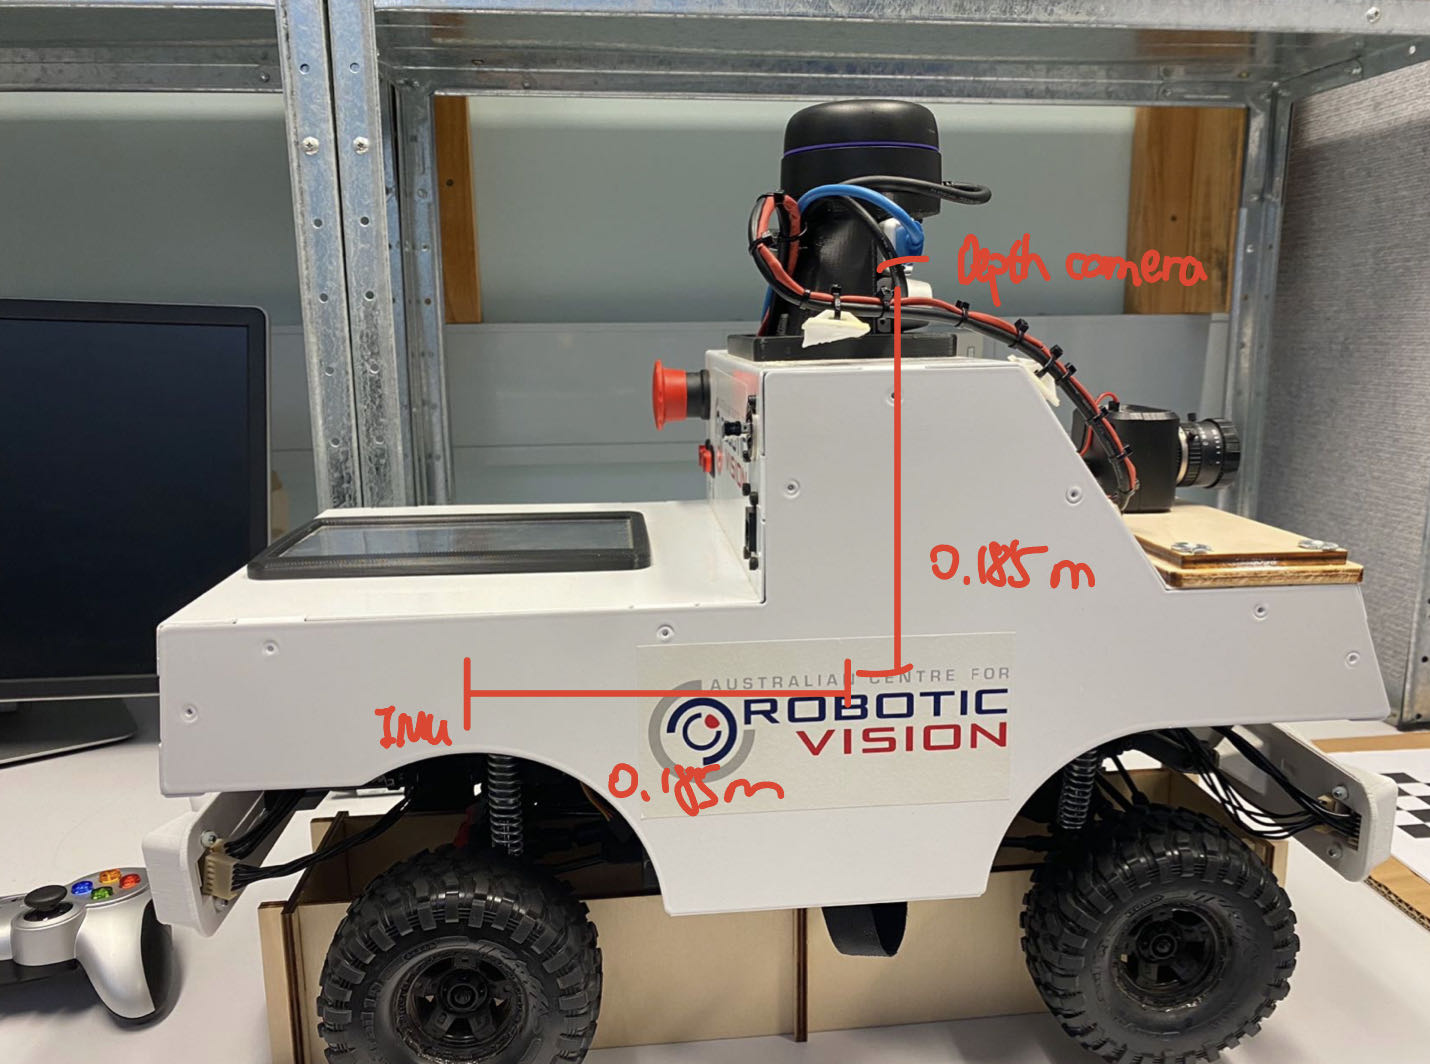
\includegraphics[width=\textwidth]{newlabel.jpeg}
        \caption{Layout of the ACRV car}
        \label{fig:first_image}
    \end{subfigure}
    \hfill
    \begin{subfigure}[b]{0.45\textwidth}
        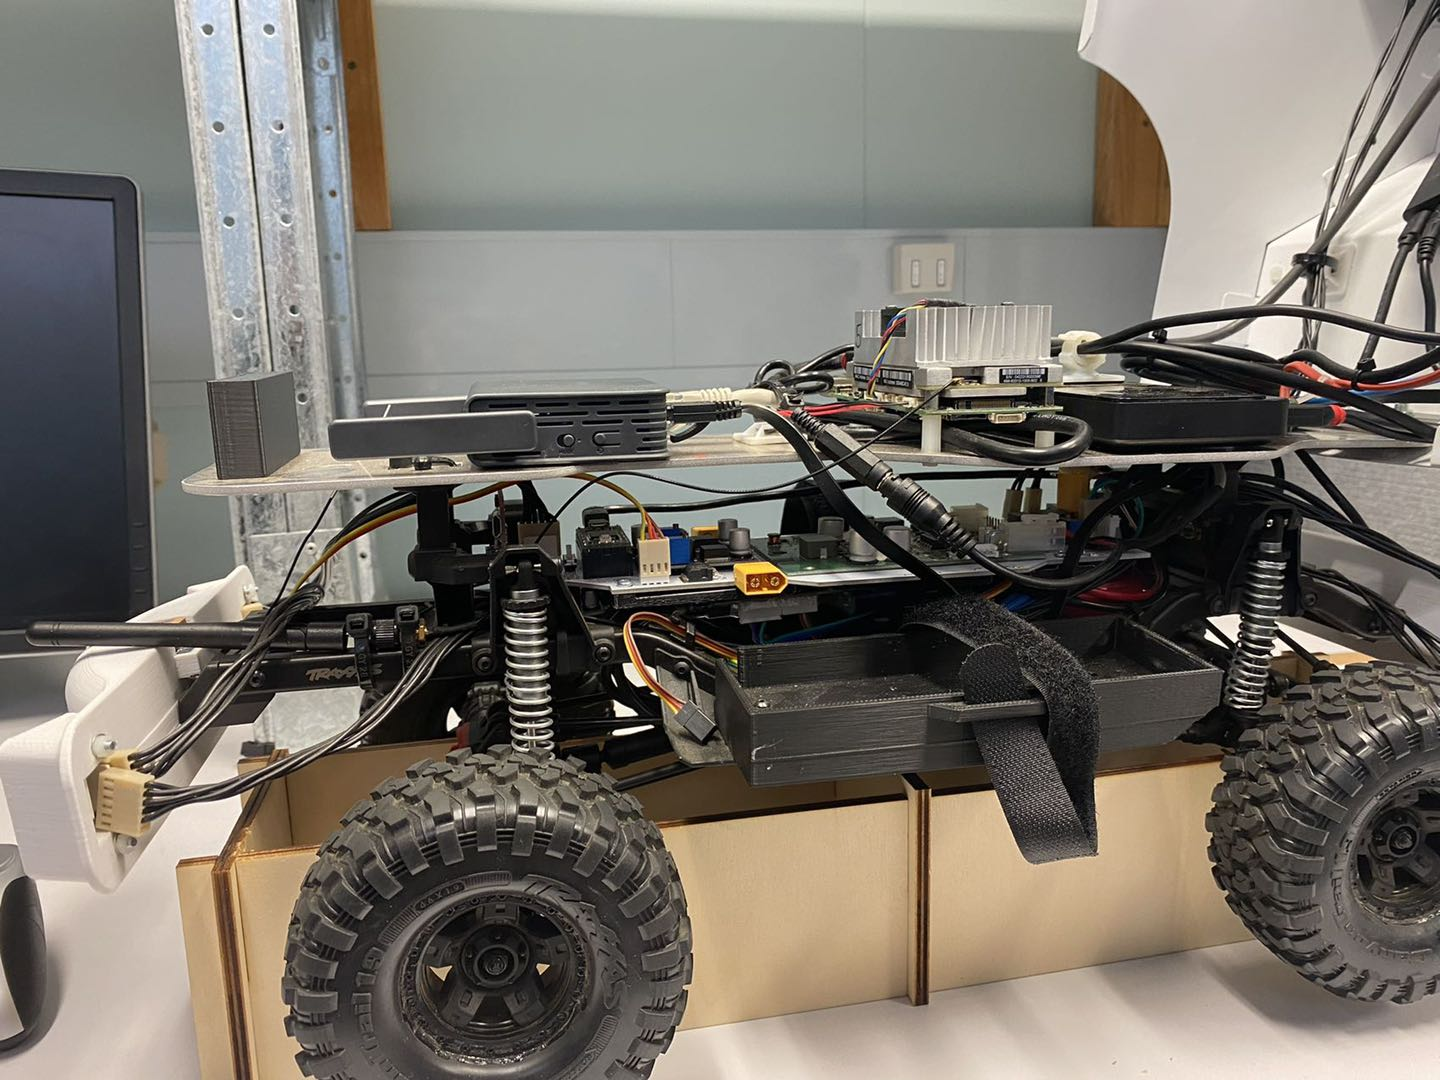
\includegraphics[width=\textwidth]{inside.jpeg}
        \caption{Inner structure of the ACRV car}
        \label{fig:second_image}
    \end{subfigure}
    \caption{Car layout(left) and car inner structure(right)}
    \label{fig:both_images}
\end{figure}
\noindent
From the figure 1, the general layout of the car is shown, the camera is 
at front end of the car, where IMU lies at the near end of the car. As usual, the
camera is placed with z axis pointing forward, and y and x axis pointing dowanward 
and out of page, the detailed orientation is shown in figure 2 in next section.
For the camera and imu frame, we simply assume they are perfectly aligned, and 
the rotation matrix consists of zero and one only.


\section*{IMU Frame and Rotation Estimation}
Next, we estimate the IMU frame, 
since only the postion of IMU is determined. To figure out
the frame of imu, we do estimation
by driving the car forward and backward. 
This motion allows us to identify 
the Z-axis of the IMU frame as 
it points forward in the direction of the car's movement.
\begin{figure}[H]
    \centering
    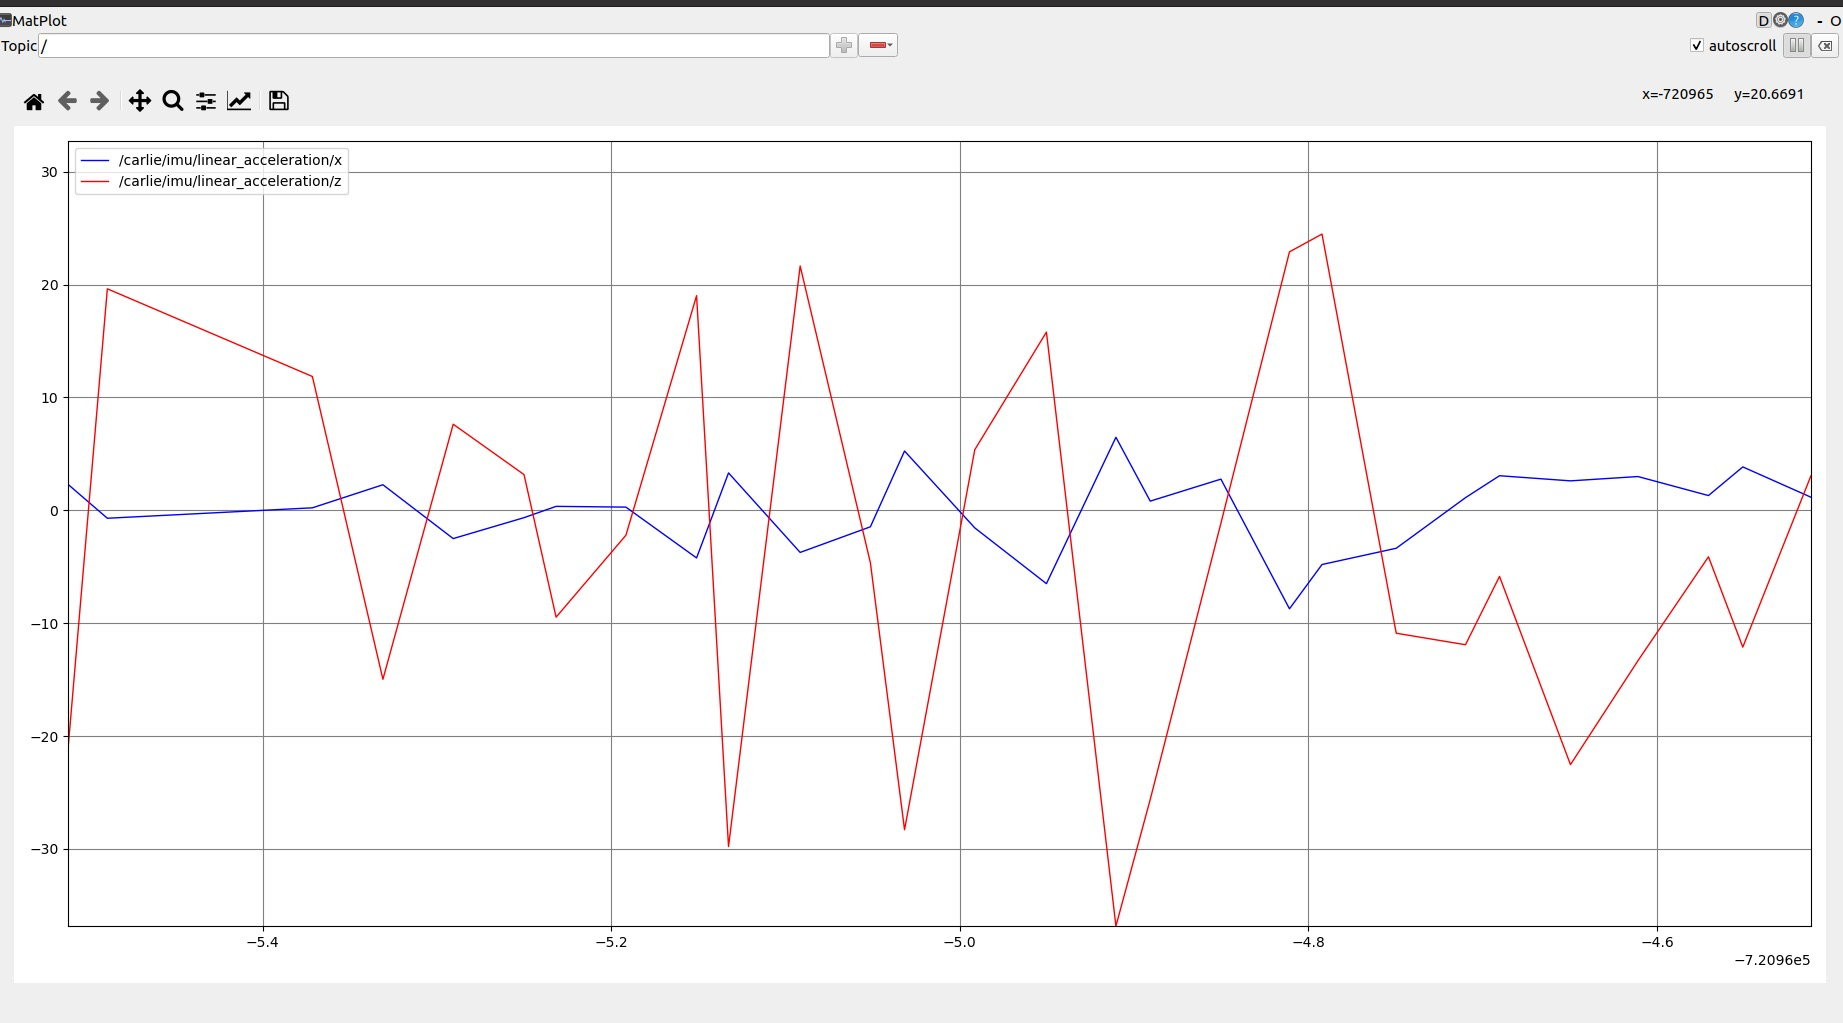
\includegraphics[width=0.5\textwidth]{imuplot.jpeg}
    \caption{Plot of imu while driving car forward}
    \label{fig:IMU plot}
\end{figure}
\noindent
As shwon in the previous plot, as car is driving forward, the z axis is varying frequently.
 Additionally, since the Y-axis of the IMU frame has a measurement of 10 by echoing 
 the rostopic message, we can deduce that it is pointing upward. 
 With this information, we can determine the complete IMU coordinate frame, and we can conclude
 that the z axis is pointing forward of the car frame, y axis is pointing upward and x axis pointing 
 into the page, as stated in figure 3 in next section.
\noindent
To estimate the IMU rotation, we examine the orientation of the IMU relative to the camera frame. 
By comparing the orientation data of the camera and IMU, we can compute the rotation matrix that aligns the IMU 
frame with the camera frame. This rotation matrix is crucial for fusing the IMU and camera data in applications 
like visual-inertial odometry and SLAM.
where the rotation matirx of camera with respect to IMU position is: 
\begin{equation}
    I_{R_C} = 
    \begin{aligned}[b]
        \begin{bmatrix}
            -1 & 0 & 0 \\
            0 & -1 & 0 \\
            0 & 0 & 1
        \end{bmatrix}
    \end{aligned}
\end{equation}

\begin{figure}[H]
    \centering
    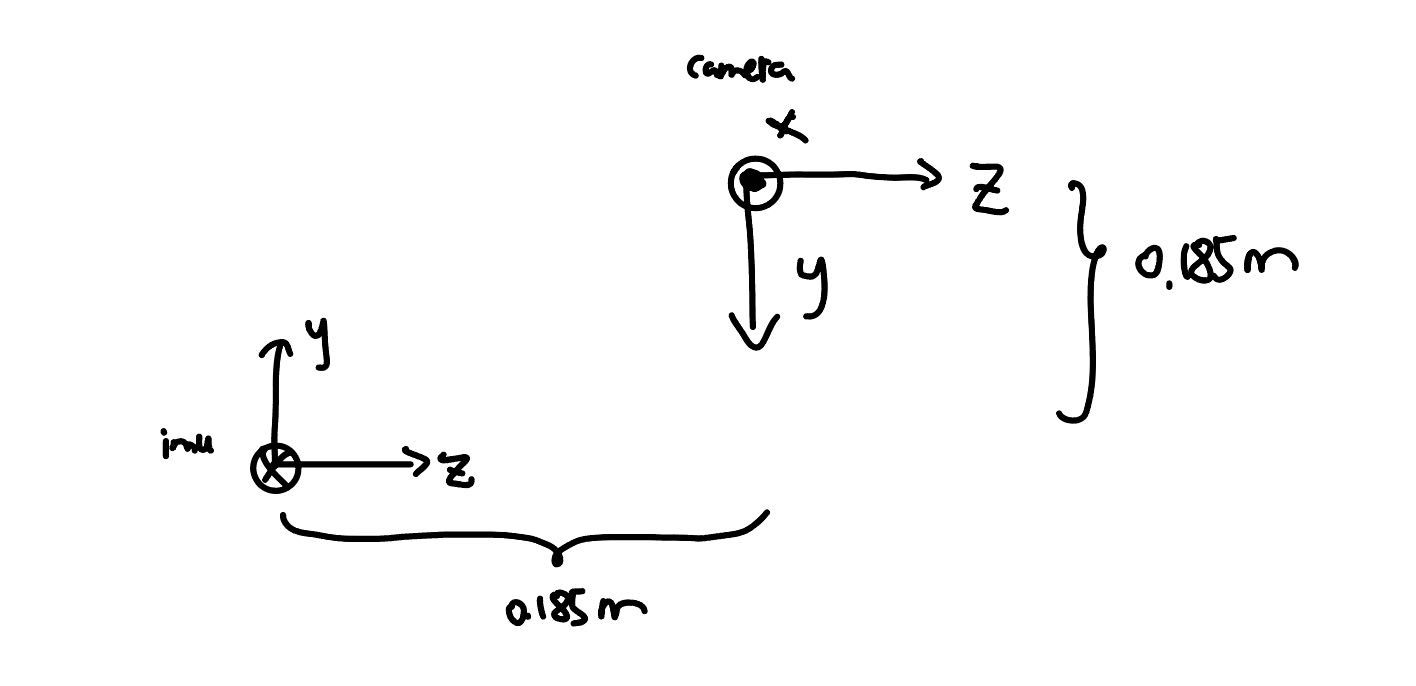
\includegraphics[width=1\textwidth]{imu_layout.jpeg}
    \caption{Relative postion of camera w.r.t IMU}
    \label{fig:IMU pos}
\end{figure}

\section*{IMU translation Estimation}
By measuring the position of the camera and the position of the IMU at the end of the car, 
we can estimate the translation vector between the IMU and camera frames. 
This translation vector is necessary for transforming 
measurements from the IMU frame to the camera frame or vice versa.
\begin{equation}
    I_{P_C} = 
    \begin{aligned}[b]
        \begin{bmatrix}
            0     \\
            0.185  \\
            0.185 
        \end{bmatrix}
    \end{aligned}
\end{equation}
Combined the information of the rotation and translation of camera and IMU,
the extrinsic provided to the camera config will be:
\begin{equation}
    I_{X_C} =
    \begin{aligned}[b]
        \begin{bmatrix}
            -1 & 0 & 0 &0\\
            0 & -1 & 0 &0.185\\
            0 & 0 & 1  &0.185\\
            0 & 0& 0& 1
        \end{bmatrix}
    \end{aligned}
\end{equation}


\section*{Camera Cabration-OpenCV}
Finally, we utilize the OpenCV Python library to perform camera calibration. 
OpenCV provides a comprehensive set of functions for camera calibration, 
including functions for estimating intrinsic and extrinsic parameters, 
correcting lens distortion, and calculating reprojection errors. 
By following the standard OpenCV camera calibration pipeline, 
we obtain the calibration results, 
including the intrinsic and extrinsic parameters of the camera.
\newline
In the ACRV car, the depth camera is pin hole model, 
the pinhole camera model is a simple geometric representation 
of the imaging process of a camera. In this model, 
light rays pass through a single point (the pinhole) 
and project onto an image plane. 
The basic idea behind the pinhole camera model 
is that a 3D point in the world can be projected onto a 
2D image plane through a single point, which is the focal point of the camera.
\newline
The equation shown above represents the transformation from world coordinates 
(X, Y, Z) to image coordinates (u, v) using intrinsic and extrinsic camera parameters. 
The intrinsic parameters include the focal length $(f_x, f_y)$ and the principal point ($c_x, c_y)$, 
which determine how the 3D points are projected onto the 2D image plane. 
The extrinsic parameters consist of a rotation matrix (R) and 
a translation vector (t) that describe the relationship 
between the world and camera coordinate systems.
\newline
In the pinhole camera model, 
the intrinsic and extrinsic parameters are combined into 
a single 3x4 projection matrix P, which is the product 
of the intrinsic matrix K and the extrinsic matrix $[R | t]$:

\begin{equation*}
    P = K [R | t] =
    \begin{bmatrix}
    f_x & 0 & c_x \\
    0 & f_y & c_y \\
    0 & 0 & 1
    \end{bmatrix}
    \begin{bmatrix}
    r_{11} & r_{12} & r_{13} & t_1 \\
    r_{21} & r_{22} & r_{23} & t_2 \\
    r_{31} & r_{32} & r_{33} & t_3
    \end{bmatrix}
    \begin{bmatrix}
        X \\
        Y \\
        Z \\
        1
    \end{bmatrix}
\end{equation*}
\noindent
By multiplying the world coordinates (X, Y, Z, 1) 
with the projection matrix P, 
we obtain the homogeneous image coordinates (s, u, v, 1). 
To obtain the pixel coordinates (u, v), 
we need to divide u and v by the scale factor s.
\newline
The camera calibration process aims to estimate 
the intrinsic and extrinsic parameters of the camera, 
which can be used to correct for lens distortion, 
determine the relationship between pixel coordinates 
and real-world coordinates, and calculate reprojection errors. 
By using OpenCV and a set of 2D-3D correspondences 
(e.g., from images of a checkerboard pattern), 
we can obtain accurate estimates of the camera parameters 
and the confidence of results.

\subsection*{1. Acquiring Calibration Images}
A set of images containing a checkerboard pattern, 
is captured from various angles and distances,
all the edges are captured, and the checkerboard is (8,6).
These images serve as the input for the calibration process.

\subsection*{2. Detecting Pattern Corners}
For each calibration image, 
OpenCV detects the corners of the checkerboard pattern. 
These corners serve as the 2D image points 
required for calibration. 
In addition, the corresponding 3D object points, 
which represent the real-world coordinates 
of the corners, are defined.

\subsection*{3. Estimating Camera Parameters}
Using the detected 2D image points and the corresponding 3D object points, 
OpenCV estimates the camera's intrinsic parameters. 
The intrinsic parameters include the camera matrix, 
which contains the focal lengths and the principal point, 
and the distortion coefficients, 
which describe the radial and tangential lens distortions. 
The extrinsic parameters describe the rotation and translation of 
the camera with respect to the real-world scene,which is already shown above in previous 
section.

\subsection*{4. Calculating Reprojection Errors}
Reprojection errors provide a measure of the accuracy of the estimated camera parameters. 
To calculate the reprojection errors, 
the 3D object points are projected back onto the 
image plane using the estimated camera parameters. 
The differences between the reprojected 
points and the original 2D image points are then calculated. 
The reprojection errors can be visualized using a scatter plot, 
where each point represents the error 
in the x and y coordinates of a reprojected point.

\begin{figure}[H]
    \centering
    \begin{subfigure}[b]{0.45\textwidth}
        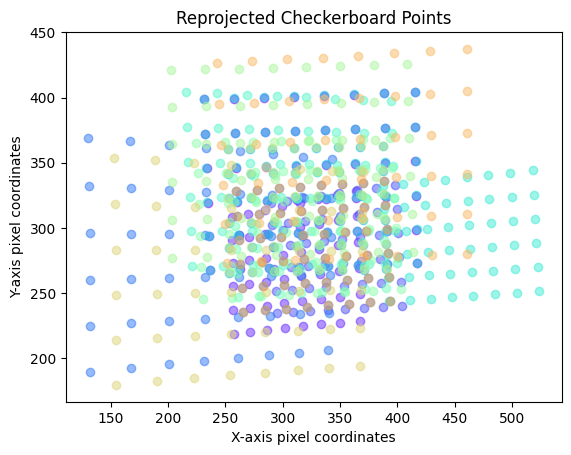
\includegraphics[width=\textwidth]{reprojection.png}
        \caption{Reprojections of the images}
        \label{fig:reprojection}
    \end{subfigure}
    \hfill
    \begin{subfigure}[b]{0.45\textwidth}
        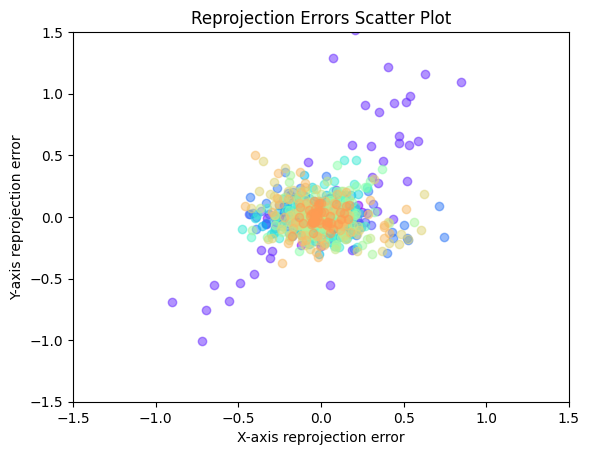
\includegraphics[width=\textwidth]{error.png}
        \caption{Reprojection in x axis and y axis}
        \label{fig:error}
    \end{subfigure}
    \caption{Reprojection error}
    \label{fig:overall_reprojection}
\end{figure}
\noindent
As shown above, in Figure 4(a), the reprojected image point is shown in the plot,
each image is taken in different angles and all the edges are involved. 
\newline
Figure 4(b)
shows the reprojection error of each images' projected point with respect to the 
real points in checkerboard, as we can seen the overall error is in side $\pm 1.5$ in both
y and x axis, which shows the calibration result is relatively accurate.
\newline
The camera matrix and distortion coefficients are:
\begin{equation*}
    \text{Camera matrix} = 
    \begin{bmatrix}
        651.25357417 &   0&         327.92109969\\
        0&         652.46869878& 221.92884596\\
        0&           0&           1        
    \end{bmatrix}
\end{equation*}

\begin{equation*}
    \text{Distortion coefficient} = 
    \begin{bmatrix}
        0.123 & 0.938 & -0.022 & -0.002 & -4.056
    \end{bmatrix}
\end{equation*}



\subsection*{5. Refining Camera Parameters}
If the reprojection errors are large, 
the calibration process can be refined by adjusting 
the initial estimates of the camera parameters and repeating the calibration. 
This process can be iterated until the reprojection errors are minimized.

\subsection*{6. Correcting Lens Distortion}
Once the camera parameters have been estimated, 
the captured images can be undistorted using OpenCV's 
functions for correcting lens distortion. 
This step is crucial for many computer vision tasks, 
as it ensures that the images accurately represent the real-world scene.

\section*{Conclusion}
In conclusion, by estimating the camera frame, 
IMU frame, IMU rotation, IMU translation, 
and calculating the reprojection error, 
we effectively calibrate the camera and IMU. 
This calibrated setup not only provides accurate 
intrinsic and extrinsic parameters but also helps 
in assessing the quality of the calibration through 
the reprojection error. The lower the reprojection error, 
the better the calibration. 
The calibrated setup allows for accurate data 
fusion between the camera and IMU, 
enabling applications such as visual-inertial odometry, 
simultaneous localization and mapping (SLAM), 
and other robotics tasks that require 
precise knowledge of the sensor's relative positions and orientations.

\end{document}
